\subsection{Training}
We train the neural network using pantheon data. The pantheon data is split into train and test data in equal size randomly. 512 datapoints are used for training and remaiing for testing. The network architecture is described in previous section. We use meansquared error loss and adam optimizer, with early stopping technique to prevent overfitting. Dropout technique with $dropout_rate$ = 0.2. The hyperparameters used are $batch_size$ = 10, $learning_rate$ = 1e-3, $patience$ = 5.
\begin{figure}[H]
	\centering
	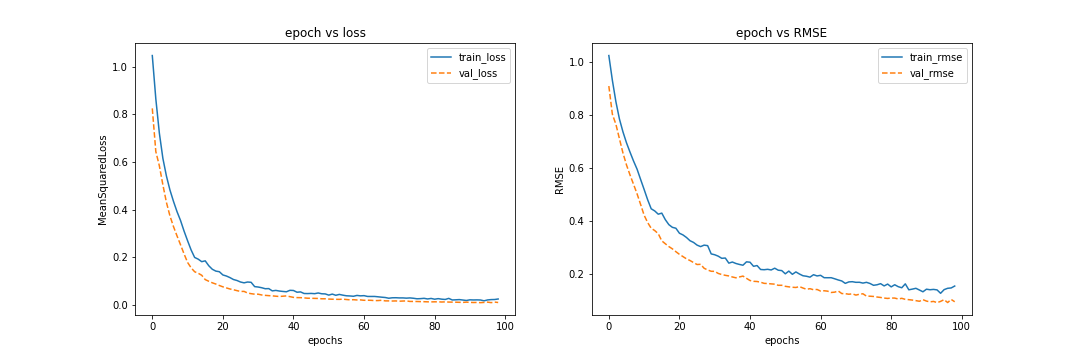
\includegraphics[width=\textwidth]{pantheon/lstm/05_epoch_vs_loss.png}
	\caption{Loss curve}
	\label{fig:loss_curve}
\end{figure}
\begin{figure}[H]
	\centering
	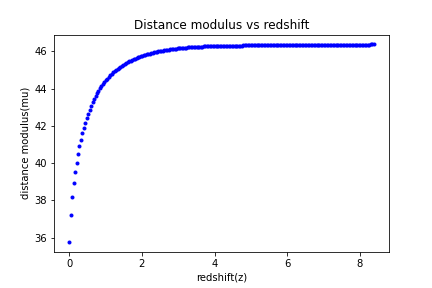
\includegraphics[width=0.8\textwidth]{pantheon/lstm/06_sample_reconstruction.png}
	\caption{Loss curve}
	\label{fig:reconstruction}
\end{figure}